\documentclass[tikz,convert={density=300,outext=.png}]{standalone}
\usetikzlibrary{arrows.meta,graphs}
\begin{document}
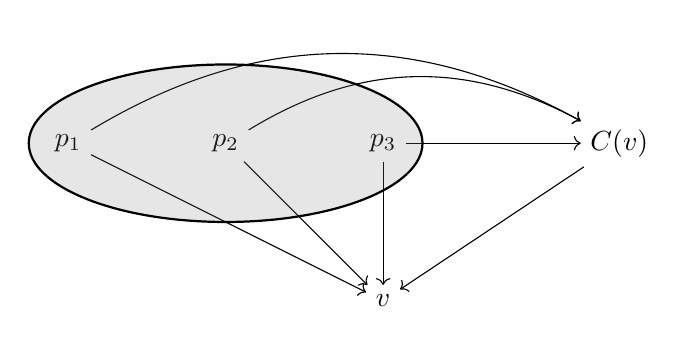
\begin{tikzpicture}
    \node (a) at (0,0) {$p_1$};
    \node (b) at (2,0) {$p_2$};
    \node (c) at (4,0) {$p_3$};
    \node (d) at (4,-2) {$v$};
    \node (e) at (7,0) {$C(v)$};
  \graph[use existing nodes] {
    a -> d;
    b -> d;
    c -> d;
    e -> d;
    a ->[bend left] e;
    b ->[bend left] e;
    c -> e;
  };
  \draw[fill=gray, fill opacity = 0.2, draw=black, thick] (2,0) ellipse (2.5cm and 1cm);
\end{tikzpicture}
\end{document}
